\documentclass[fleqn]{beamer}

\usepackage[british]{babel}
\usepackage{graphicx,ru,url}
\graphicspath{{./figures/}}
\usepackage{amsmath}
% Use Times for math font and text font.
\RequirePackage[T1]{fontenc}
%\RequirePackage{txfonts}
% bold math must be loaded after Times font
\usepackage{bm}
\usepackage{booktabs} % nice rules (thick lines) for tables
\usepackage{microtype} % improves typography for PDF
\usepackage{xcolor} % Allows colors in fonts

\usepackage{tikz} % Allows creation of tikz pictures
\usetikzlibrary{arrows}
\usetikzlibrary{arrows.meta}

\usepackage{verbatim}
\usetikzlibrary{arrows,shapes,snakes}
\usetikzlibrary{patterns}
\usepackage{url}
\usepackage{ifthen}
\usepackage{subcaption}
\usepackage{slashbox} % backslashbox in a table

% typesetting using the algorithmicx package
% detail at: https://en.wikibooks.org/wiki/LaTeX/Algorithms and https://tex.stackexchange.com/questions/229355/algorithm-algorithmic-algorithmicx-algorithm2e-algpseudocode-confused
\usepackage{algorithm}
\usepackage{algpseudocode}

\usepackage{multibib}
\newcites{Mypub}{List of Publications}

% The title of the presentation:
%  - first a short version which is visible at the bottom of each slide;
%  - second the full title shown on the title slide;
\title[Modeling of TREAT Detectors]{
    Modeling and Simulation of Neutron Detectors for the Transient REActor Test (TREAT) Facility}

% Optional: a subtitle to be displayed on the title slide
%\subtitle{Show where you're from}

% The author(s) of the presentation:
%  - again first a short version to be displayed at the bottom;
%  - next the full list of authors, which may include contact information;
\author[Wenkai Fu]{
    Wenkai Fu\\
    Advisor: Prof.~Jeremy Roberts}

% The institute:
%  - to start the name of the university as displayed on the top of each slide
%    this can be adjusted such that you can also create a Dutch version
%  - next the institute information as displayed on the title slide
\institute[Kansas State University]{
    Department of Mechanical and Nuclear Engineering \\
    Kansas State University}

% Add a date and possibly the name of the event to the slides
%  - again first a short version to be shown at the bottom of each slide
%  - second the full date and event name for the title slide
\date[Ph.D. Defense]{
    Ph.D. Defense\\
    Ward Hall 135\\
    April 19, 2019}

\begin{document}
    % These two commands allow bonus slides at the end
    % The bonus slides will not be numbered
    \newcommand{\beginbackup}{
        \newcounter{framenumbervorappendix}
        \setcounter{framenumbervorappendix}{\value{framenumber}}
    }
    \newcommand{\backupend}{
        \addtocounter{framenumbervorappendix}{-\value{framenumber}}
        \addtocounter{framenumber}{\value{framenumbervorappendix}}
    }
    
    \begin{frame}
        \titlepage
    \end{frame}

    \begin{frame}
     \frametitle{Outline}
      \begin{itemize}
       \item Overview of TREAT Facility
       \item Out-of-core hodoscope detectors
       
       \begin{itemize}
        \item ZnS(Ag) scintillation detectors
        \item Fast-sensitive Microstructured Semiconductor Neutron Detectors (MSNDs)
       \end{itemize}
       \item In-core Micro-Pocket Fission Detector (MPFD)
       \item Conclusion
%        \item *Fuel motion device for burnup measurements
      \end{itemize}
    \end{frame}

    \section{TREAT Overview}
    
    \begin{frame}
       \frametitle{Overview of Transient REActor Test (TREAT) Facility}
       \begin{columns}[c]
        \begin{column}{.5\textwidth}
         \begin{figure}
        \includegraphics[width = \textwidth]{key_component_treat.jpg}
        \caption{TREAT Facility \cite{bess2015baseline}.}
       \end{figure}
        \end{column}
        \begin{column}{.5\textwidth}
          \begin{tabular}{ll}
          \toprule
          Max. neutron flux & $10^{17}$~cm$^{-2}$s$^{-1}$\\
          Max. core power & 19~GW \\ %\cite{imholte2016comparison}\\
          Shutdown & April 1994\\
          \multicolumn{2}{l}{Fast nuclear fuels}\\
          Restart & 9/18/2018\\
          \multicolumn{2}{l}{Accident Tolerant Fuels (ATFs)}\\
          \bottomrule
         \end{tabular}
        \end{column}
       \end{columns}
    \end{frame}
    
   \section{Hodoscope Detectors}
   \begin{frame}
    \frametitle{TREAT Hodoscope}
    \begin{figure}
        \includegraphics[width = \textwidth, trim={0, 3cm, 0, 6cm}, clip]{hodoscope_image}
        \caption{Schematic of TREAT hodoscope \cite{treat_hodoscope_image}.}
       \end{figure}
   \end{frame}

    \begin{frame}
     \frametitle{TREAT Hodoscope: Radiation Environment}
      \begin{equation*}
      \begin{split}
 N(E) &\propto \mbox{exp}(-E / 0.988) \sinh(\sqrt{2.249 E})\\
 G(E) &= \left\{ \begin{array}{ll}
                 38.13 (E - 0.085) e^{1.648E} & E < 0.3\\
                 26.8 e^{-2.3E} & 0.3 < E < 1.0\\
                 8.0e^{-1.1E} & 1.0 < E < 8.0
                \end{array} \right.
      \end{split}
      \end{equation*}
      
     \begin{columns}[c]
      \begin{column}{.5\textwidth}
       \begin{tabular}{ll}
      \toprule
      Signal & Noise\\
      \midrule
       Neutron & Gamma\\
       $N_n = 1$ & $N_\gamma = 10$ \cite{de1975fast}\\
       Monodirectional & Isotropic\\
       \bottomrule
      \end{tabular}
      \end{column}

      \begin{column}{.5\textwidth}
      \includegraphics[width = \textwidth]{ng_spec}
      \end{column}
     \end{columns}
    \end{frame}
    
    \begin{frame}
    \begin{itemize}
     \item ZnS(Ag) scintillation detectors
     \begin{itemize} 
      \item Hornyak button
      \item Layered detector
     \end{itemize}
    \end{itemize}
    \end{frame}

    \begin{frame}
     \frametitle{ZnS(Ag) Scintillation Detectors: Physics}
     \begin{columns}[c]
      \begin{column}{.5\textwidth}
         \begin{figure}
     \centering
      \includegraphics[width = \textwidth]{hornyak_button}
%       \caption{Schematic of Hornyak button fast neutron detector \cite{ghosh2018high}.}
     \end{figure}
     PMMA: (C$_5$O$_2$H$_8$)$_n$, 1.19~g/cm$^3$
      \end{column}

      \begin{column}{.5\textwidth}
      \resizebox{\textwidth}{!}{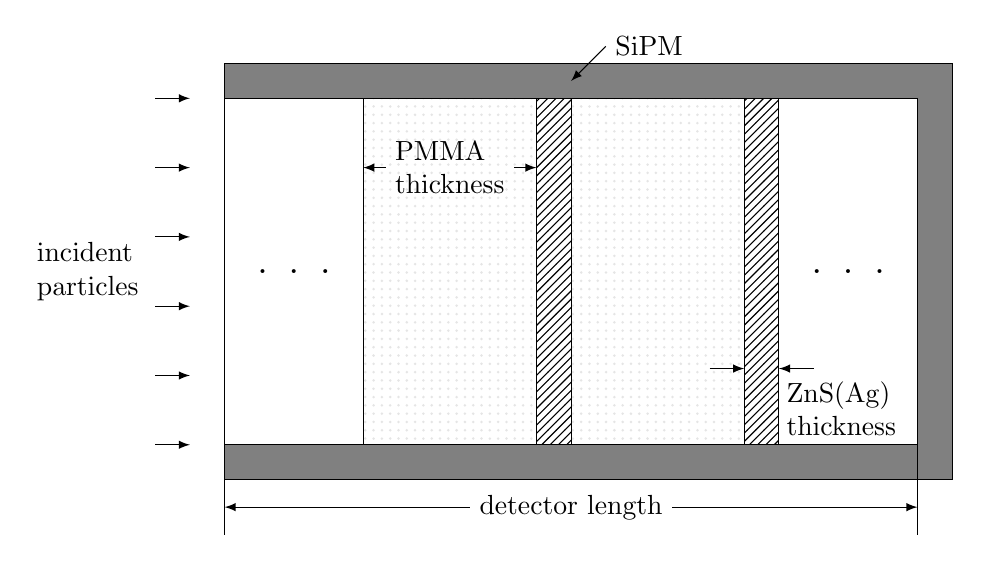
\begin{tikzpicture}[scale = .44, >=latex]
\def\zsa{1}
\def\pmma{5}
\def\height{10}
\draw [fill = gray] (0, 0) rectangle (21, 12);
\draw [<-] (10, 11.5) -- (11, 12.5) node [right] {SiPM};

\draw [fill = white] (0, 1) rectangle (20, 11);
\draw [<->] (0, -.8) -- (20, -.8) node [midway, fill = white] {detector length};
\draw (20, 1) -- (20, -1.6);
\draw (0, 1) -- (0, -1.6);

\draw [pattern = dots, pattern color=black!10!white] (4, 1) rectangle (4 + \pmma, 11);
\draw [<->] (4, 9) -- (4 + \pmma, 9) node [midway, preaction =  {fill=white},pattern=dots,pattern color=black!10!white, align=left] {PMMA\\thickness};
\draw [pattern = dots, pattern color=black!10!white] (4 + \pmma + \zsa, 1) rectangle (4 + \pmma + \pmma + \zsa, 11);

\draw [pattern = north east lines] (4 + \pmma, 1) rectangle (4 + \pmma + \zsa, 11);

\draw [pattern = north east lines] (4 + \pmma+ \pmma + \zsa, 1) rectangle (4 + \pmma + \zsa+ \pmma + \zsa, 11);
\draw [->] (4 + \pmma+ \pmma + \zsa - 1, 3.2) -- (4 + \pmma+ \pmma + \zsa, 3.2);
\draw [<-] (4 + \pmma + \zsa+ \pmma + \zsa, 3.2) -- (4 + \pmma + \zsa+ \pmma + \zsa + 1, 3.2);
\node [below, align = left] at (4 + \pmma + \zsa+ \pmma + \zsa + 1.8, 3.1) {ZnS(Ag)\\thickness};

\node [thick] at (2,6) {\LARGE . . .};
\node [thick] at (18, 6) {\LARGE. . .};

\foreach \x in {0, 1, ..., 5}
\draw [->] (-2, 1+\x*2) -- (-1, 1+\x*2);
\node [left, align=left] at (-2.2, 6) {incident\\particles};
\end{tikzpicture}}
%       \begin{flushleft}
%       detection efficiency: 0.4\%\\suffered from Cherenkov noise \cite{de1975fast}
%       \end{flushleft}
      \end{column}
     \end{columns}
     \vspace{.5cm}
     Objectives:
     \begin{itemize}
      \item Reduce Cherenkov noise
      \item Neutron detector efficiency (NDE) larger than 0.4\% \cite{de1975fast}
     \end{itemize}
     \end{frame}
     
     \begin{frame}
      \centering
      Geant4 Hornyak Button Model
     \end{frame}

     
     \begin{frame}
      \frametitle{Hornyak Button: ZnS(Ag) Grain Randomization}
      \begin{columns}[c]
       \begin{column}{.5\textwidth}
        \begin{tabular}{ll}
         $\rho_{zsa}$ & 4.09\\
         $\rho_{PMMA}$ & 1.19\\
         weight ratio & 5\%\\
         $r_{zsa}$ & 20~$\mu$m \cite{fink1982optimization}\\
         $N_g$ & $\boxed{\approx 5\times10^5}$
        \end{tabular}
        \textcolor{white}{hello}\\
        \textcolor{white}{hello}
        
        \begin{tikzpicture}
         \draw  (0, 0) -- (5, 0);
         \foreach \x in {0, .5, ..., 5}{
         \draw [dashed] (\x, -.2) -- (\x, .2);
         }
         \draw (.1, -.3) -- (.1, .3) node [above] {$c_g$};
         \draw (.75, -.3) -- (.75, .3) node [above] {$c_g$};
         \draw (1.45, -.3) -- (1.45, .3) node [above] {$c_g$};
        \end{tikzpicture}
       \end{column}

       \begin{column}{.5\textwidth}
      \begin{figure}[h!tb]
\centering
\begin{subfigure}{.8\textwidth}
\centering
\includegraphics[width = \textwidth, trim = {4cm, 6cm, 0, 3cm}, clip]{overall}
\label{fig:hb1}
\end{subfigure}
\begin{subfigure}{.8\textwidth}
\centering
\includegraphics[width = \textwidth]{xz_zoom_zoom}
\label{fig:hb2}
\end{subfigure}
\caption{Randomization of ZnS(Ag) grains.}
\label{hb_g4}
\end{figure}
       \end{column}
      \end{columns}
     \end{frame}
     
     \begin{frame}
      \frametitle{Hornyak Button: Optical Properties and Sources}
      \begin{columns}[c]
       \begin{column}{.5\textwidth}
       \centering
        \resizebox{\textwidth}{!}{\begin{tabular}{ll}
        \toprule
       Scintillation yield (keV$^{-1}$) & 37\\
       Optical MFP in ZnS(Ag) ($\mu$m) & 13\\
       Emission spectrum peak (nm) & 450$^v$\\
       ZnS(Ag) refractive index & 2.36\\
       PMMA refractive index & 1.49$^v$\\
       Non-PMT surfaces & reflective\\
       PMT surface & polished\\
       ZnS(Ag) grain surface & ground\\
       \bottomrule
      \end{tabular}}
       \end{column}

       \begin{column}{.5\textwidth}
        \begin{figure}
\def\scale{3}
\centering
\begin{subfigure}{.6\textwidth}
\centering
\begin{tikzpicture}
[scale = \scale]
\def\lenx{5./8.}
\def\leny{7. / 64.}
\def\radius{3. / 8.}
\def\angle{10}
\draw [pattern = dots] (-\lenx / 2., -\leny / 2.) rectangle (\lenx / 2., \leny / 2.);
\draw [thick] (\radius, \leny / 2.) arc [radius = 0.38078, start angle = \angle, end angle = 180 - \angle];
\draw [thick] (-\radius, \leny / 2.) -- (\radius, \leny / 2.);
\draw [thick] (\radius, -\leny / 2.) arc [radius = 0.38078, start angle = 350, end angle = 190];
\draw [thick] (-\radius, -\leny / 2.) -- (\radius, -\leny / 2.);
\end{tikzpicture}
\caption{one neutron}
\end{subfigure}

\begin{subfigure}{.6\textwidth}
\centering
\begin{tikzpicture}[scale = \scale]
\def\lenx{5./8.}
\def\leny{7. / 64.}
\def\radius{3. / 8.}
\draw [pattern = dots] (-\lenx / 2., -\leny / 2.) rectangle (\lenx / 2., \leny / 2.);
\draw [thick, pattern = dots] (\radius, \leny / 2.) arc [radius = 0.38078, start angle = 10, end angle = 170];
\draw [thick] (-\radius, \leny / 2.) -- (\radius, \leny / 2.);
\draw [thick, pattern = dots] (-\radius, -\leny / 2.) arc [radius = 0.38078, start angle = 190, end angle = 350];
\draw [thick] (-\radius, -\leny / 2.) -- (\radius, -\leny / 2.);
\end{tikzpicture}
\caption{69 gamma rays}
\end{subfigure}
\end{figure}
       \end{column}
      \end{columns}
     \end{frame}
     
     \begin{frame}
      \frametitle{Hornyak Button: Pulse Height Distribution}
      \begin{figure}
       \includegraphics[width = .5\textwidth]{pulse_height_hb}
       \includegraphics[width = .5\textwidth]{neff_hb}
       \caption{At S/N ratio of 100, NDE is 0.35\% considering the  scintillation noise. If Cherenkov noise is included, the efficiency reduces to 0.086\%.}
      \end{figure}
     \end{frame}

     \begin{frame}
     \centering
      Geant4 Layered Detector Model
     \end{frame}

%      \begin{frame}
%       \frametitle{Layered Detector: Physics}
%       \begin{figure}
%       \centering
%        \resizebox{.8\textwidth}{!}{\begin{tikzpicture}[scale = .44, >=latex]
% \def\zsa{1}
% \def\pmma{5}
% \def\height{10}
% \draw [fill = gray] (0, 0) rectangle (21, 12);
% \draw [<-] (10, 11.5) -- (11, 12.5) node [right] {SiPM};
% 
% \draw [fill = white] (0, 1) rectangle (20, 11);
% \draw [<->] (0, -.8) -- (20, -.8) node [midway, fill = white] {detector length};
% \draw (20, 1) -- (20, -1.6);
% \draw (0, 1) -- (0, -1.6);
% 
% \draw [pattern = dots, pattern color=black!10!white] (4, 1) rectangle (4 + \pmma, 11);
% \draw [<->] (4, 9) -- (4 + \pmma, 9) node [midway, preaction =  {fill=white},pattern=dots,pattern color=black!10!white, align=left] {PMMA\\thickness};
% \draw [pattern = dots, pattern color=black!10!white] (4 + \pmma + \zsa, 1) rectangle (4 + \pmma + \pmma + \zsa, 11);
% 
% \draw [pattern = north east lines] (4 + \pmma, 1) rectangle (4 + \pmma + \zsa, 11);
% 
% \draw [pattern = north east lines] (4 + \pmma+ \pmma + \zsa, 1) rectangle (4 + \pmma + \zsa+ \pmma + \zsa, 11);
% \draw [->] (4 + \pmma+ \pmma + \zsa - 1, 3.2) -- (4 + \pmma+ \pmma + \zsa, 3.2);
% \draw [<-] (4 + \pmma + \zsa+ \pmma + \zsa, 3.2) -- (4 + \pmma + \zsa+ \pmma + \zsa + 1, 3.2);
% \node [below, align = left] at (4 + \pmma + \zsa+ \pmma + \zsa + 1.8, 3.1) {ZnS(Ag)\\thickness};
% 
% \node [thick] at (2,6) {\LARGE . . .};
% \node [thick] at (18, 6) {\LARGE. . .};
% 
% \foreach \x in {0, 1, ..., 5}
% \draw [->] (-2, 1+\x*2) -- (-1, 1+\x*2);
% \node [left, align=left] at (-2.2, 6) {incident\\particles};
% \end{tikzpicture}}
% \caption{The MLFD is designed to reduce Cherenkov noise (using SiPM to collect light) and to increase neutron detection efficiency (the layered configuration). The cross section area is a $2.52 \times 8.89$~mm rectangle.}
%       \end{figure}
%      \end{frame}

\begin{frame}
 \frametitle{Layered Detector: Thickness Optimization}
 \begin{table}[h!tb]
\caption{The NDEs (\%) of 5-cm long, layered detectors with different layer thicknesses. The LLDs were set to achieve S/N ratio of 100 considering scintillation and Cherenkov noises.} 
\label{layer_opt}
\resizebox{\textwidth}{!}{\begin{tabular}{l|lllllll}
\toprule
\backslashbox{PMMA~(mm)}{ZnS(Ag)~($\mu$m)} & 2 &4 &7 &12 &21 &35 & 59 \\
\midrule
0.10 & 2.05 & 3.02 & 3.15 & 2.49 & 2.21 & & \\
0.18 & 2.44 & 3.03 & 3.26 & \textbf{3.31} & 2.71 & 2.06 & \\
0.32 & & 2.16 & 2.47 & 2.54 & 2.61 & 2.43 & 2.11 \\
\bottomrule
\end{tabular}}
\end{table}
\end{frame}

\begin{frame}
 \frametitle{Layered Detector: Pulse Height Distribution}
 \begin{figure}
       \includegraphics[width = .5\textwidth]{layer_5cm_ph}
       \includegraphics[width = .5\textwidth]{layer_5cm_neff}
       \caption{PHDs and NDEs of the 5-cm long, best-case layered detector.}
      \end{figure}
\end{frame}

\begin{frame}
 \frametitle{Layered Detector: Length Evaluation}
 \begin{figure}
  \includegraphics[width = .65\textwidth]{length_test_layer}
  \caption{NDEs of the layered detectors with different lengths.}
 \end{figure}
\end{frame}

\begin{frame}
\centering
\begin{itemize}
 \item Fast-Sensitive Microstructured Semiconductor Neutron Detectors (MSNDs)
 \begin{itemize}
  \item Actinide
  \item Hydrogenous
 \end{itemize}
\end{itemize}
\end{frame}

\begin{frame}
 \frametitle{Fast-Sensitive MSNDs: Physics}
 \begin{figure}[h!tb]
\centering
\def\trench{1.6}
\def\wall{1}
\def\top{9.5}
\def\bot{3}
\def\pcontact{0.2}

\resizebox{.75\textwidth}{!}{
\begin{tikzpicture}[scale = 0.38, >=latex]
\draw (0, 0) rectangle (\wall + 6 * \trench + 6 * \wall, 10);
% au contacts
\draw [fill = black] (0, 0) rectangle (\wall + 6 * \trench + 6 * \wall, -0.3);
\draw [fill = black] (0, \top + \pcontact) rectangle (\wall + \pcontact, 10);
\draw [fill = black] (\wall * 7 + 6 * \trench, 10) rectangle (\wall * 7 + 6 * \trench - \wall - \pcontact, \top + \pcontact);

% n-type contact
\draw [fill = black!10!white] (0.5, 0) rectangle (\wall + 6 * \trench + 6 * \wall - 0.5, 0.5);

\draw [pattern = north west lines] (0, \top) -- (\wall, \top) -- (\wall, \bot) -- (\trench + \wall, \bot) -- (\trench + \wall, \top) -- (\trench + 2*\wall, \top) -- (\trench + 2 * \wall, \bot) -- (2 * \trench + 2 * \wall, \bot) -- (2 * \trench + 2 * \wall, \top) -- (2 * \trench + 3 * \wall, \top) -- (2 * \trench + 3 * \wall, \bot) -- (3 * \trench + 3 * \wall, \bot) -- (3 * \trench + 3 * \wall, \top) -- (3 * \trench + 4 * \wall, \top) -- (3 * \trench + 4 * \wall, \bot) -- (4 * \trench + 4 * \wall, \bot) -- (4 * \trench + 4 * \wall, \top) -- (4 * \trench + 5 * \wall, \top) -- (4 * \trench + 5 * \wall, \bot) -- (5 * \trench + 5 * \wall, \bot) -- (5 * \trench + 5 * \wall, \top) -- (5 * \trench + 6 * \wall, \top) -- (5 * \trench + 6 * \wall, \bot) -- (6 * \trench + 6 * \wall, \bot) -- (6 * \trench + 6 * \wall, \top) -- (6 * \trench + 7 * \wall, \top) -- (6 * \trench + 7 * \wall, 10) -- (0, 10) -- (0, \top); 

% p-type contact
\draw [fill = gray] (0, \top) -- (\wall, \top) -- (\wall, \bot) -- (\trench + \wall, \bot) -- (\trench + \wall, \top) -- (\trench + 2*\wall, \top) -- (\trench + 2 * \wall, \bot) -- (2 * \trench + 2 * \wall, \bot) -- (2 * \trench + 2 * \wall, \top) -- (2 * \trench + 3 * \wall, \top) -- (2 * \trench + 3 * \wall, \bot) -- (3 * \trench + 3 * \wall, \bot) -- (3 * \trench + 3 * \wall, \top) -- (3 * \trench + 4 * \wall, \top) -- (3 * \trench + 4 * \wall, \bot) -- (4 * \trench + 4 * \wall, \bot) -- (4 * \trench + 4 * \wall, \top) -- (4 * \trench + 5 * \wall, \top) -- (4 * \trench + 5 * \wall, \bot) -- (5 * \trench + 5 * \wall, \bot) -- (5 * \trench + 5 * \wall, \top) -- (5 * \trench + 6 * \wall, \top) -- (5 * \trench + 6 * \wall, \bot) -- (6 * \trench + 6 * \wall, \bot) -- (6 * \trench + 6 * \wall, \top) -- (6 * \trench + 7 * \wall, \top) -- 
(6 * \trench + 7 * \wall, \top + \pcontact) -- (6 * \trench + 6 * \wall - \pcontact, \top + \pcontact) -- (6 * \trench + 6 * \wall - \pcontact, \bot + \pcontact) -- (6 * \wall + 5 * \trench + \pcontact, \bot + \pcontact) -- (6 * \wall + 5 * \trench + \pcontact, \top + \pcontact) -- (5 * \wall + 5 * \trench - \pcontact, \top + \pcontact) -- (5 * \wall + 5 * \trench - \pcontact, \bot + \pcontact) -- (5 * \wall + 4 * \trench + \pcontact, \bot + \pcontact) -- (5 * \wall + 4 * \trench + \pcontact, \top + \pcontact) -- (4 * \wall + 4 * \trench - \pcontact, \top + \pcontact) -- (4 * \wall + 4 * \trench - \pcontact, \bot + \pcontact) -- (4 * \wall + 3 * \trench + \pcontact, \bot + \pcontact) -- (4 * \wall + 3 * \trench + \pcontact, \top + \pcontact) -- (3 * \wall + 3 * \trench - \pcontact, \top + \pcontact) -- (3 * \wall + 3 * \trench - \pcontact, \bot + \pcontact) -- (3 * \wall + 2 * \trench + \pcontact, \bot + \pcontact) -- (3 * \wall + 2 * \trench + \pcontact, \top + \pcontact) -- (2 * \wall + 2 * \trench - \pcontact, \top + \pcontact) -- (2 * \wall + 2 * \trench - \pcontact, \bot + \pcontact) -- (2 * \wall + \trench + \pcontact, \bot + \pcontact) -- (2 * \wall + \trench + \pcontact, \top + \pcontact) -- (\wall + \trench - \pcontact, \top + \pcontact) -- (\wall + \trench - \pcontact, \bot + \pcontact) -- (\wall + \pcontact, \bot + \pcontact) -- (\wall + \pcontact, \top + \pcontact) -- (0, \top + \pcontact) -- (0, \top);

% label
\draw [<-] (1, 0.25) -- (-1, 1) node [left, align = left] {n-type\\contact};
\draw [<-] (\wall + 0.5 * \pcontact, \top -3) -- (-1, \top-1) node [left, align = left] {p-type\\contact};
\draw [<-] (\wall + 0.5 * \trench, \top + 0.1) -- (\wall + 0.5 * \trench + 0.2, \top + 0.1 + 1) node [above, align=left] {neutron\\converter};
\draw [<-] (\wall * 3 + 2.5 * \trench, \top - 1.5) -- (\wall * 3 + 2.5 * \trench + 0.5, \top + 0.1 + 1) node [above] {trench};
\draw [<-] (\wall * 4.5 + 4 * \trench, \top - 1.5) -- (\wall * 4.5 + 4 * \trench + 0.5, \top + 1.1) node [above] {wall};
\node at (\wall * 3.5 + 3 * \trench, 1.5) {n-type Si};
\draw [<->] (\wall * 7 + \trench * 6 + 0.5, 10) -- (\wall * 7 + \trench * 6 + 0.5, \bot) node [midway, right, align=left] {etch\\depth};
\draw [<-] (7 * \wall + 6 * \trench - 0.5 * \wall, 10) -- (7 * \wall + 6 * \trench - 0.5 * \wall - 0.5 * \trench, \top + 1.1) node [above] {Au contact};
% length label
\draw [<->] (0, -1.2) -- (\wall + 6 * \trench + 6 * \wall, -1.2) node [midway, fill = white] {length};
% trench wall width label
\draw [<->] (\wall, \bot-\pcontact) -- (2 * \wall + \trench, \bot-\pcontact) node [below, midway] {T + W};

% neutron
\draw [fill = blue] (\wall * 4 + 3.5 * \trench, 0.5 * \top + 0.5 * \bot) circle [radius = 0.2];
\draw [<-] (\wall * 4 + 3.5 * \trench, 0.5 * \top + 0.5 * \bot + 0.2) -- (\wall * 4 + 3.5 * \trench, \top + 1.1) node [above] {n};
\draw [fill = red, red] (\wall * 3.5 + 3 * \trench, 0.8 * \top) circle [radius = 0.2];
\draw [fill = red, red] (\wall * 4.5 + 4 * \trench, 0.53 * \top) circle [radius = 0.2];
\draw [->, thick, red] (\wall * 4 + 3.5 * \trench, 0.5 * \top + 0.5 * \bot) -- (\wall * 3.5 + 3 * \trench, 0.8 * \top);
\draw [->, thick, red, dashed] (\wall * 4 + 3.5 * \trench, 0.5 * \top + 0.5 * \bot) -- (\wall * 4.5 + 4 * \trench, 0.53 * \top);

% bulk Si
\draw [dashed, teal, ultra thick] (0, 0) rectangle (\wall + 6 * \trench + 6 * \wall, \bot);
\node [teal, right, align = center] at (\wall + 6 * \trench + 6 * \wall, \bot / 2) {bulk\\Si};

\end{tikzpicture}}
\caption{MSND physics, where T and W are the trench and wall widths, respectively.}
\label{msnd}
\end{figure}
\end{frame}

 \begin{frame}
  \frametitle{Fast-Sensitive MSNDs: Cross Sections}
  \begin{block}{Thermal-sensitive MSND}
     \begin{equation*}
      ^6 \mbox{Li} + _0^1 n \rightarrow ^4\mbox{He} (2.07 \mbox{MeV}) + ^3\mbox{H}(2.73 \mbox{MeV})
     \end{equation*}
%      $\sigma_t = 937$~b; $\Sigma_t = 114.60$~cm$^{-1}$
    Detection efficiency of DS-MSND is 69\% \cite{ochs2018improved}
    \end{block}
    
    \begin{block}{Cross sections of the fast-neutron converters.}
\resizebox{\textwidth}{!}{
\begin{tabular}{lllll}
\toprule
Converter & Density (g/cm$^3$) & Molecular weight (g/mole) & $\overline{\sigma}$ (b) & $\overline{\Sigma}$ (cm$^{-1}$) \\
\midrule
paraffin wax (C$_{25}$H$_{52}$) & 0.93 & 352.68 & 3.93 & 0.32 \\
$^{237}$Np & 20.25 & 237.05 & 1.31 & 0.067 \\
$^{235}$U & 18.95 & 235.04& 1.21 & 0.059  \\
$^{238}$U & 18.95 & 238.05& 0.31 & 0.015 \\
$^{232}$Th & 11.72 & 232.04& 0.075 & 0.0023 \\
\bottomrule
\end{tabular}}
    \end{block}
 \end{frame}
 
 \begin{frame}
  \frametitle{Fast-Sensitive MSND: Source}
  \begin{figure}
    \centering
    \resizebox{.75\textwidth}{!}{
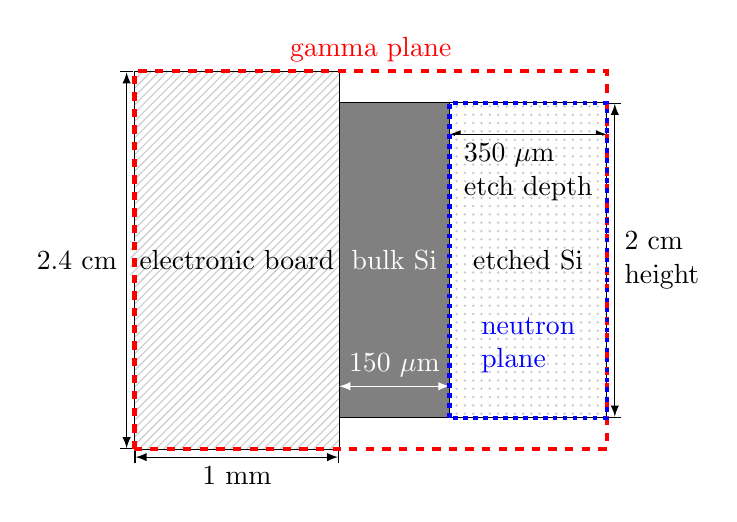
\begin{tikzpicture}[scale = 2, >=latex]
\def\elecD{1.3}
\def\bulkSiD{0.7}
\def\trenchD{1}
\def\offset{0.05}

% elec. board
\draw [pattern = north east lines, pattern color = black!20!white] (0, 0) rectangle (\elecD, 2.4) node [pos = 0.5, align = left, preaction = {fill = white}, pattern = north east lines, pattern color = black!20!white] {electronic board};
\draw [|<->|] (0, -\offset) -- (\elecD, -\offset) node [midway, below] {1~mm};
\draw [|<->|] (-\offset, 0) -- (-\offset, 2.4) node [midway, left] {2.4~cm};

% bulk Si
\draw [fill = gray] (\elecD, 0.2) rectangle (\elecD+\bulkSiD, 2.2) node [pos = 0.5, align = left, white] {bulk Si};
\draw [<->, white] (\elecD, 0.4) -- (\elecD + \bulkSiD, 0.4) node [white, midway, above] {150~$\mu$m};


% etched Si
\draw [pattern = dots, pattern color=black!20!white] (\elecD+\bulkSiD, 0.2) rectangle (\elecD+\bulkSiD+\trenchD, 2.2) node [pos=.5, align = left]{etched Si};
% depth
\draw [<->] (\elecD + \bulkSiD, 2) -- (\elecD + \bulkSiD + \trenchD, 2) node [below, midway, preaction =  {fill=white}, pattern = dots, pattern color=black!20!white, align = left] {350~$\mu$m\\etch depth};
% height
\draw [|<->|] (\elecD + \bulkSiD + \trenchD + \offset, 0.2) -- (\elecD + \bulkSiD + \trenchD + \offset, 2.2) node [midway, right, align = left] {2 cm\\height};


% source plane
% gamma
\draw [dashed, red, ultra thick] (0, 0) rectangle (\elecD + \bulkSiD + \trenchD, 2.4);
\node  [above, red] at (1.5, 2.4) {gamma plane};
% neutron
\draw [dotted, blue, ultra thick] (\elecD + \bulkSiD, 0.2) rectangle (\elecD + \bulkSiD + \trenchD, 2.2);
\node [below, blue, align = left] at (\elecD + \bulkSiD + \trenchD * 0.5, 0.9) {neutron\\plane};
\end{tikzpicture}}

\caption{$N_n : N_\gamma = 1 : 51$.}
\end{figure}
  \end{frame}
 
 \begin{frame}
  \frametitle{Fast-Sensitive MSND: Source (cont.)}
  \begin{figure}
  \centering
  \includegraphics[width = \textwidth, trim = {0, 7cm, 3cm, 3cm}, clip]{ng_source}
  \caption{Neutron and gamma sources.}
  \end{figure}
 \end{frame}

 
 
 \begin{frame}
 \centering
  Geant4 actinide MSND Model
 \end{frame}


 
 \begin{frame}
  \frametitle{Actinide MSND: Width Optimization}
  \begin{figure}
\centering
\includegraphics[width = .5\textwidth]{U235_tw}
\includegraphics[width = .5\textwidth]{spectrum}
\caption{The NDE of the 2-cm long, $^{235}$U-filled MSND with 20-$\mu$m trench and 10-$\mu$m wall widths is 1.2\% at 5-MeV LLD.}
\end{figure}
 \end{frame}
 
 \begin{frame}
  \frametitle{Actinide MSND: Length Evaluation}
  \begin{figure}[h!tb]
\centering
\includegraphics[width = .7\textwidth]{actinide_length}
\caption{NDEs of actinide MSNDs with different lengths.}
\label{actinide_length}
\end{figure}
 \end{frame}
 
 \begin{frame}
 \centering
  Geant4 hydrogenous MSND model
 \end{frame}

 
 \begin{frame}
  \frametitle{Hydrogenous MSND: Width Optimization}
  \begin{table}[h!tb]
\caption{NDEs (\%) of the 2-cm long hydrogenous MSNDs with different trench and wall widths. Shown in parentheses are LLDs in MeV that achieve S/N ratio of 100.}
\label{tw_hmsnd_gamma}
\resizebox{\textwidth}{!}{\begin{tabular}{l|lllll}
\toprule
\backslashbox{Trench ($\mu$m)}{Wall ($\mu$m)} &  25 & 30 & 40 & 50 & 60 \\
\midrule
40 & 2.01 (1.225) & 2.21 (1.250) & 2.21 (1.325)\\
50 & & 2.37 (1.175) & 2.20 (1.300) & 2.15 (1.350) \\
60 & 2.04 (1.125) & 2.28 (1.150) & \textbf{2.47 (1.200)} & 2.29 (1.275) & 2.04 (1.350)\\
70 & & 2.35 (1.100) & 2.41 (1.175) & 2.25 (1.250) & 2.11 (1.300)\\
80 & & 2.18 (1.100) & 2.36 (1.150) & 2.32 (1.200) & 2.09 (1.275)\\
90 & & & 2.30 (1.125) & 2.20 (1.200) & 2.11 (1.250)\\
100 & & & 2.18 (1.125) & 2.15 (1.200) & 2.14 (1.200)\\
\bottomrule
\end{tabular}}
\end{table}
 \end{frame}
 
 \begin{frame}
  \frametitle{Hydrogenous MSND: Pulse Height Distribution}
  \begin{figure}[h!tbp]
\centering
\includegraphics[ width = .7\textwidth]{hmsnd_gn_spectrum}
\caption{PHDs of the best-case 2-cm long hydrogenous MSND.}
\label{ng_spectra}
\end{figure}
 \end{frame}
 
 \begin{frame}
  \frametitle{Hydrogenous MSND: Length Evaluation}
  \begin{figure}[h!tb]
\centering
\includegraphics[ width = .7\textwidth]{neff_sn100}
\caption{NDEs of the hydrogenous MSNDs with different lengths.}
\label{gamma_length}
\end{figure}
 \end{frame}
 
%  \begin{frame}
%   \frametitle{Hydrogenous MSND: Fabrication}
%   \begin{figure}
%    \centering
%    \includegraphics[width = .65\textwidth]{hmsnd}
%    \caption{The scanning electron microscope image of the hydrogenous MSND filled with paraffin wax.}
%   \end{figure}
% 
%  \end{frame}


 \section{MPFD}
 \begin{frame}
 \centering
  Micro-Pocket Fission Detector (MPFD), Explored
 \end{frame}
 
 \begin{frame}
  \frametitle{MPFD: Physics}
  \centering
%   \resizebox{.7\textwidth}{!}{
  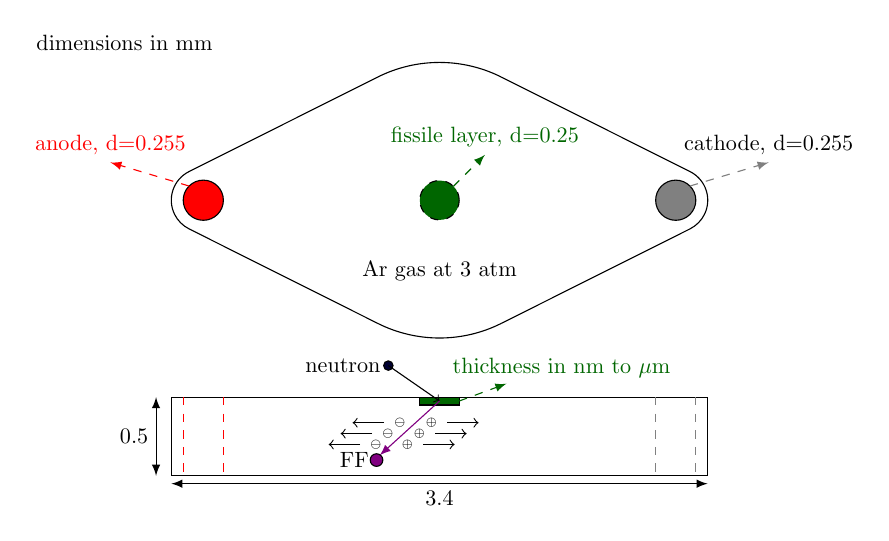
\begin{tikzpicture}[scale = 2, every node/.style={scale=.8}, >=latex] % , every node/.style={scale=10}
       % cross section view
       \coordinate (c1) at (-1.5, 0);
       \coordinate (c2) at (1.5, 0);
       \coordinate (p2) at (-1.591, -.1817);
       \coordinate (p4) at (-.3919, -.7823);
       \coordinate (p5) at (.3919, -.7823);
       \coordinate (p7) at (1.591, -.1817);
       \coordinate (p8) at (1.591, 0.1817);
       \coordinate (p9) at (.3919, 0.7823);
       \coordinate (p10) at (-.3919, 0.7823);
       \coordinate (p3) at (-1.591, .1817);
       
       % unit label
       \node at (-2, 1) {dimensions in mm}; 
       
       \draw (p3) arc (90 + 26.603:270-26.603:.2032); % left arc
       \draw (p2) -- (p4);
       \draw (p10) arc (90+26.609:90-26.609:.875);   % upper arc
       \draw (p5) -- (p7);
       \draw (p8) -- (p9);
       \draw (p8) arc (90 - 26.603:26.603-90:.2032); % right arc
       \draw (p4) arc (270-26.609:270+26.609:.875);  % lower arc
       \draw (p3) -- (p10);
       
       % wire
       \draw [fill=red] (c1) circle (.255/2);
       \draw [fill = gray] (c2) circle (.255/2);
       
       % fisile layer
       \draw [dashed, fill = green!40!black] (0, 0) circle (.25 / 2);
       \pgfmathsetmacro{\x}{cos(45)}
%        \draw [-{Latex[length=3mm, width=.5mm]}, dashed, green!40!black] (.25/2*\x, .25 / 2 * \x) -- (.25/2*\x + .2, .25 / 2 * \x + .2) node [right, above] {fissile layer, d=0.25};
       \draw [>=latex, ->, dashed, green!40!black] (.25/2*\x, .25 / 2 * \x) -- (.25/2*\x + .2, .25 / 2 * \x + .2) node [right, above] {fissile layer, d=0.25};
       
       % electrode label
       \draw [->, dashed, red] (-1.59, 0.09) -- (-1.59 - .5, 0.09 + .15) node [left, above] {anode, d=0.255};
       \draw [->, dashed, gray] (1.59, 0.09) -- (1.59 + .5, 0.09 + .15) node [right, above, black] {cathode, d=0.255};
      
       % Ar
       \node at (0, -.45) {Ar gas at 3 atm};
       
       % -------------------------------------
       % height view
       % -------------------------------------
       \def\yshift{.25}
       \draw (-1.7032, -1 - \yshift) rectangle (1.7032, -1.5 - \yshift);
%        \draw [{Latex[length=3mm, width=.5mm]}-{Latex[length=3mm, width=.5mm]}] (-1.7032, -1.55) -- (1.7032, -1.55) node [midway, below] {3.4};
       \draw [<->, >= latex] (-1.7032, -1.55 - \yshift) -- (1.7032, -1.55-\yshift) node [midway, below] {3.4};
       \draw [<->, >= latex] (-1.8, -1 - \yshift) -- (-1.8, -1.5 - \yshift) node [left, midway] {0.5};
       
       % wires
       \draw [dashed, red] (-1.5 - .255/2, -1- \yshift) -- (-1.5 - .255/2, -1.5- \yshift);
       \draw [dashed, red] (-1.5 + .255/2, -1- \yshift) -- (-1.5 + .255/2, -1.5- \yshift);
       \draw [dashed, gray] (1.5 - .255/2, -1- \yshift) -- (1.5 - .255/2, -1.5- \yshift);
       \draw [dashed, gray] (1.5 + .255/2, -1- \yshift) -- (1.5 + .255/2, -1.5- \yshift);
       
       % fissile layer
       \draw [fill = green!40!black] (-.25/2, -1- \yshift) rectangle (.25 / 2, -1.05- \yshift);
       \draw [>=latex, ->, dashed, green!40!black] (.25 / 2, -1.025- \yshift) -- (.25 / 2 + .3, -1.025 + .11- \yshift) node [right, above] at (.25 / 2 + .65, -1.025 + .1 - \yshift) {thickness in nm to $\mu$m};
       
       % neutron
       \draw [fill = blue!20!black] (-.25/2 - .2, -1- \yshift + .2) circle (.03) node [left] {neutron};
       \draw [->, >=to] (-.25/2 - .2, -1- \yshift + .2) -- (0, -1.025 - \yshift);
       
       % FF
       \draw [->, >=latex, violet] (0, -1.025 - \yshift) -- (-.38, -1.62);
       \draw [fill = violet] (-.4, -1.4 - \yshift) circle (.04) node [left] {FF};
       
       % charge carrier
       \pgfmathsetmacro{\dx}{-.38 / 5}
       \pgfmathsetmacro{\k}{(-1.62 + 1.025 + .25) / -.38}
       \pgfmathsetmacro{\b}{-1.025 - .25}
       \foreach \i in {2, 3, 4}{
       \node at (\dx * \i + .1, \k * \dx * \i + \b) {\text{\tiny $\oplus$}};
       \draw [->, >=to] (\dx * \i + .2, \k * \dx * \i + \b) -- (\dx * \i + .4, \k * \dx * \i + \b);
       \node at (\dx * \i - .1, \k * \dx * \i + \b) {\text{\tiny $\ominus$}};
       \draw [->, >=to] (\dx * \i -.2, \k * \dx * \i + \b) -- (\dx * \i - .4, \k * \dx * \i + \b);
       }
      \end{tikzpicture}
 \end{frame}

 \begin{frame}
  \frametitle{MPFD: Computational Routine \cite{garfield_elmer_example}}
\centering
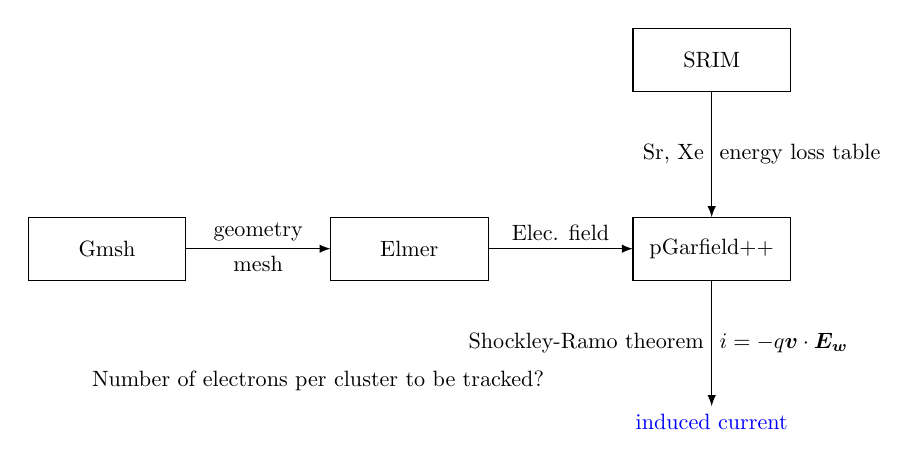
\begin{tikzpicture}[>=latex, scale = .8, every node/.style={scale=.8}]
      % origin at left and lower coner of the Garfield box
      \def\width{2.5}
      \def\height{1}
      \def\aspace{2}
       \draw (0, 0) rectangle (\width, \height) node at (\width / 2, \height / 2) {pGarfield++};
       \draw [->] (\width / 2, 0) -- (\width / 2, -\aspace) node [below] {\textcolor{blue}{induced current}}
       node [left] at (\width / 2, -\aspace / 2) {Shockley-Ramo theorem};
       \node [right] at (\width / 2, -\aspace / 2) {$i = -q \boldsymbol{v} \cdot \boldsymbol{E_w}$};
       
       \draw (0, \height + \aspace) rectangle (\width, 2 * \height + \aspace) node at (\width / 2, 1.5 * \height + \aspace) {SRIM};
       \draw [->] (\width / 2, \height + \aspace) -- (\width / 2, \height) node [right] at (\width/2, \height + \aspace / 2) {energy loss table} node [left] at (\width/2, \height + \aspace / 2) {Sr, Xe};
       
       \def\aspace{2.3}
       \draw (-\aspace - \width, 0) rectangle (-\aspace, \height) node at (-\aspace - \width / 2, \height / 2) {Elmer};
       \draw [->] (-\aspace, \height / 2) -- (0, \height / 2) node [above] at (-\aspace / 2, \height / 2) {Elec. field};
       
       \draw (-2*\width - 2 * \aspace, 0) rectangle (-\width - 2 * \aspace, \height) node at (-2 * \aspace - 1.5 * \width, \height / 2) {Gmsh};
       \node at (-2 * \width, -1.6 * \height) {Number of electrons per cluster to be tracked?};
       \draw [->] (-\width - 2 * \aspace, \height / 2) -- (-\width - \aspace, \height / 2) node [above] at (-\width - 1.5 * \aspace, \height / 2) {geometry} node [below] at (-\width - 1.5 * \aspace, \height / 2) {mesh};
      \end{tikzpicture}
 \end{frame}
 
 \begin{frame}
  \frametitle{MPFD: Electron Tracking Algorithms}
  \begin{columns}[c]
   \begin{column}{.5\textwidth}
    \begin{block}{Monte Carlo integration}
     A table contains
     \begin{itemize}
      \item drift velocity
      \item longitudinal and transverse diffusion coefficients
      \item attachment coefficients
      \item Townsend coefficients
     \end{itemize}
     as a function of electric field.
     
     
     \begin{itemize}
      \item[$\ast$] electric field grids?
      \item[$\ast$] number of collisions?
     \end{itemize}
    \end{block}
   \end{column}
   
   \begin{column}{.5\textwidth}
    \begin{block}{Microscopic tracking $\surd$}
    Electron scattering rates stored in Magboltz database
    \begin{itemize}
     \item elastic
     \item ionization
     \item attachment
     \item inelastic
     \item excitation
     \item super-elastic
     \item[--] phonon-related scatterings
     \item[--] coulomb scattering
    \end{itemize}

    \end{block}
   \end{column}


  \end{columns}

 \end{frame}



\begin{frame}
 \frametitle{MPFD: Electric Field}
 \begin{columns}[c]
  \begin{column}{.5\textwidth}
  \begin{block}{Equations}
   \begin{equation*}
   \begin{split}
    \nabla^2 V &= -q / \varepsilon\\
    \boldsymbol{E} &= - \nabla V \, .
    \end{split}
   \end{equation*}
   \begin{tabular}{l|l}
    $V$ & electric potential\\
    $q$ & volumetric charge density\\
    $\varepsilon$ & gas permittivity\\
    $\boldsymbol{E}$ & electric field\\
    BCs & applied voltage
   \end{tabular}
   \end{block}
  \end{column}
  
  \begin{column}{.5\textwidth}
   \includegraphics[width = \textwidth, trim = {1cm, 7cm, 1cm, 7cm}, clip]{geometry}
   

   \includegraphics[width = \textwidth]{c1}
   
   \centering
   Electric field (V/cm) under 100~V applied voltage
  \end{column}
 \end{columns}
\end{frame}

\begin{frame}
 \frametitle{MPFD: Parallelization Scheme Verification}
 \begin{figure}
  \centering
  \includegraphics[width = .6\textwidth]{serial_vs_parallel_500nff_nodiff_mc}
  \caption{For performance, 500 FFs were simulated using the Monte Carlo tracking algorithm, and 0.5\% electrons per cluster were transported. Diffusion process was not simulated.}
 \end{figure}

\end{frame}


\begin{frame}
 \frametitle{MPFD: Induced Current}
 \begin{columns}[c]
 \begin{column}{.5\textwidth}
 \begin{figure}
 \centering
  \includegraphics[width = \textwidth]{micro_3c_log}
  \caption{Induced currents by three fission fragments.}
  \end{figure}
 \end{column}

  \begin{column}{.5\textwidth}
  \begin{figure}
    \centering
 \includegraphics[width = \textwidth]{micro_avg_log}
 \caption{Averaged induced current from two thousand fission fragments.}
 \end{figure}
  \end{column}

 \end{columns}
%  Garfield++ application parallelized by hybrid MPI and OpenMP.
\end{frame}

\begin{frame}
 \frametitle{MPFD: Collection Time Distribution}
 \centering
$Q = \int_0^{t_e} i(t) dt$

 \begin{columns}[c]
 \begin{column}{.5\textwidth}
  \begin{figure}
   \centering
   \includegraphics[width = \textwidth]{micro_charge_time}
   \caption{$Q$ and $t_{95}$ of the 2K FFs.}
  \end{figure}
 \end{column}

  \begin{column}{.5\textwidth}
   \begin{figure}
    \centering
    \includegraphics[width = \textwidth]{micro_t95_dist}
    \caption{$t_{95}$ distribution.}
   \end{figure}
  \end{column}
 \end{columns}
\end{frame}

\begin{frame}
 \frametitle{MPFD: Collected Charge Distribution}
 \begin{columns}[c]
  \begin{column}{.5\textwidth}
   \begin{figure}
   \centering
    \includegraphics[width = \textwidth]{micro_erg_dist}
    \caption{Distribution of deposited energy.}
   \end{figure}
  \end{column}
  
  \begin{column}{.5\textwidth}
   \begin{figure}
    \centering
    \includegraphics[width = \textwidth]{micro_charge_dist}
    \caption{Distribution of collected charge.}
   \end{figure}

  \end{column}


 \end{columns}

\end{frame}


\section{Conclusion}
\begin{frame}
 \frametitle{Conclusion}
 Neutron detectors developed for the TREAT Facility were modeled and simulated. 
 \begin{itemize}
   \item The Hornyak button model predicted neutron detection efficiency of 0.35\% and strong Cherenkov noise.
   \item Alternative hodoscope detectors were proposed and performance verified.
   \begin{itemize}
    \item A 5-cm long layered variant was predicted to have an NDE of 3.3\%.
    \item At length of 2~cm, $^{235}$U-filled and hydrogenous MSNDs were predicted to have NDEs of 1.2\% and 2.5\%, respectively.
   \end{itemize}
   
   \rule{.9\textwidth}{.2pt}
   \item A computational routine that can model the electron collection process in MPFD was developed. The induced current of in-core MPFDs was simulated to occur within 400~ns.
 \end{itemize}
\end{frame}

\begin{frame}
 \frametitle{Acknowledgements}
 \begin{itemize}
  \item Many thanks to my committee: Profs. Roberts, Andresen, Bahadori, McGregor, Shultis, and Weaver.
  \item It's my great fortune to work with my colleagues:
  \begin{itemize}
   \item CORPS: Rabab Elzohery, soon-to-be-Dr.~Richard Reed, John Boyington, Dong Lei, and Ye Cheng
   \item S.M.A.R.T.: Priyarshini Ghosh, Dan Nichols, Taylor Ochs, Dr.~Fronk,  Dr.~Reichenberger, and Dr.~Harrison
  \end{itemize}

 \end{itemize}

 
 
\end{frame}


%  \begin{frame}
%  \frametitle{Fuel Motion Device for Burnup Measurements}
%  \centering
%  \includegraphics[width = 1.1\textwidth]{fmd}
% \end{frame}

 \section{References}
    
    \begin{frame}[t,allowframebreaks]\label{lastframe}
        \frametitle{References}
        \bibliographystyle{ans}
        % make a bibliography.bib file with your references in it
        {\scriptsize
        \bibliography{bibliography}}
    \end{frame}
    
    \begin{frame}[t,allowframebreaks]
     \frametitle{Related Publications}
     \nociteMypub{*}
     \bibliographystyleMypub{ans}
     {\scriptsize
     \bibliographyMypub{mypub}}
    \end{frame}

    
\begin{frame}
 \centering
 \Large
 Thank you.\\
 Questions?
\end{frame}
\end{document}
